\documentclass[paper,oneside,onecolumn,notitlepage,bibtotocnumbered,fontsize=12pt,bigheadings,ngerman]{scrartcl}
\usepackage[singlespacing]{setspace}
\usepackage[ngerman]{babel}
\usepackage{fancyhdr}                          
\pagestyle{fancy} 
\usepackage[parfill]{parskip}                        
\addto\captionsngerman{
\renewcommand{\figurename}{Abbildung}
\renewcommand{\tablename}{Tab.}
}
\newcommand{\thema}{CAD-Project - Mom based Information Live Flow}
\newcommand{\schlagworte}{MoM, IoT, Cloud, CEP}
\newcommand{\zusammenfassung}{
}

\newcommand{\autor}{Paul Drautzburg,  Lukas Hansen,  Georg Mohr, Kim De Souza, Sebastian Thuemmel, Sascha Drobig}

%Encodingeinstellung
\usepackage[utf8]{inputenc}
%Packete zur Formatierung von Tabellen und Grafiken
\usepackage{graphicx}
\usepackage{tabularx}
\usepackage{multicol}
\usepackage{float}
\usepackage{floatflt}
\usepackage{here}
\usepackage{blindtext}
\usepackage{wrapfig}
\usepackage{bigstrut}
\usepackage{subfloat}
\usepackage{subfigure}
%\usepackage{scrpage2} 
%\pagestyle{scrheadings}
\usepackage[small]{titlesec}
\usepackage{colortbl}	
\usepackage{cite}
\usepackage{hyperref}
\usepackage{amsmath}
\usepackage{nicefrac}
\usepackage{pstricks}
\usepackage{pst-3dplot}
\usepackage{glossaries}
\usepackage{listings}
\usepackage{needspace}
\usepackage[nottoc]{tocbibind}
%\pagestyle{myheadings}
%\clearscrheadfoot
\renewcommand{\thefootnote}{\arabic{footnote}} 


%Titelseite (optional)
\newcommand{\sectionnumbering}[1]{% 
  \setcounter{section}{0}% 
   \renewcommand{\thesection}{\csname #1\endcsname{section}}} 
   
   
   
\usepackage{caption}
\DeclareCaptionFont{white}{\color{white}}
\DeclareCaptionFormat{listing}{\colorbox{gray}{\parbox{\textwidth}{#1#2#3}}}
\captionsetup[lstlisting]{format=listing,labelfont=white,textfont=white}




\usepackage{listings}


\begin{document}
\shorthandoff{"}
\pagenumbering{roman} 
\include{cover}

\include{title}

{\Large \textbf{Vorwort}}
\bigskip

Das vorliegende Dokument beschreibt die Umsetzung für das Projekt im Rahmen des MSI-Kurses \textit{Cloud Application Development}.
\include{affidavit}
\include{abstract}


\normalsize


\setlength{\parindent}{0pt}

\newpage
\sectionnumbering{Roman} 
\tableofcontents
\clearpage

\listoffigures 
\clearpage 

\listoftables 
\clearpage
\pagenumbering{arabic} 
\sectionnumbering{arabic} 

\section{Motivation}
\subsection{Zielsetzung}
ToDo: Verweis auf 12 Faktor APP Standard !!! 
Die Tabelle soll am Anfang stehen, am besten in der Zielsetzung.
Die folgende Tabelle beschreibt die Kernanforderungen der 12 Faktor APP, 
\begin{table}[!ht]
  \centering
    \begin{minipage}{15cm}
      \centering
      \begin{tabular}{*{3}{|l|p{5.0cm}|p{5.0cm}}}\hline
      \multicolumn{3}{|c|}{\cellcolor[RGB]{200,200,200}12 Faktor APP Anforderungen} \\\hline
     \textbf{ID}&\textbf{Anforderung}&\textbf{Beschreibung}\\\hline
     1.&Codebase&Eine im Versionsmanagementsystem verwaltete Codebase, viele Deployments.\\
      \hline
     2.&Abhängigkeiten&Abhängigkeiten explizit deklarieren und isolieren.\\
     \hline
     3.&Konfiguration&Die Konfiguration in Umgebungsvariablen ablegen.\\
     \hline
     4.&Unterstützende Dienste&Unterstützende Dienste als angehängte Ressourcen behandeln.\\
     \hline 
     5.&Build, release, run&Build- und Run-Phase strikt trennen.\\
     \hline
     6.&Prozesse&Die App als einen oder mehrere Prozesse ausführen.\\
     \hline
      7.&Bindung an Ports&Dienste durch das Binden von Ports exportieren.\\
     \hline
      8.&Nebenläufigkeit&Mit dem Prozess-Modell skalieren.\\
     \hline
      9.&Einweggebrauch&Robuster mit schnellem Start und problemlosen Stopp.\\
     \hline
     10.&Dev-Prod-Vergleichbarkeit&Entwicklung, Staging und Produktion so ähnlich wie möglich halten.\\
     \hline     
     11.&Logs&Logs als Strom von Ereignissen behandeln.\\
     \hline
     12.&Admin-Prozesse&Admin/Management-Aufgaben als einmalige Vorgänge behandeln.\\
     \hline
      \end{tabular}
   \caption{12 Faktor App Anforderungen}\label{tab:Anforderungen}
    \end{minipage}
\end{table}

\clearpage



\subsection{Die 12 Faktor-APP Anforderungen}

\section{Einleitung}

\section{Kommunikation der Komponenten}
Die entwickelte Anwendung besteht mit einem Java-Service für die verwendete Wetter-API, der Complex Event Processing Engine und den Anwender-Clients aus drei Komponenten. Diese Komponenten müssen möglichst stark entkoppelt miteinander kommunizieren können. Durch eine starke Entkopplung wird erreicht ,dass die jeweiligen Komponenten keine Kenntnisse über vorhandene Schnittstellen oder die verwendete Programmiersprache besitzen müssen. Um dies zu realisieren, wird RabbitMQ als Message-oriented Middleware (MoM) eingesetzt. 
\subsection{RabbitMQ}\label{rabbitmq}
Bei RabbitMQ handelt es sich um einen auf Erlang basierenden OpenSource Message Broker, welcher Bibliotheken für alle gängigen Programmiersprachen wie Java, JavaScript, Swift und C\# anbietet. Dadurch wird die Kommunikation mit Android-, iOS- und Webapplikationen möglich. Durch die Verwendung von Queues und Topics wird die asynchrone Verteilung der Nachrichten ermöglicht. RabbitMQ verwendet als Standard das Messaging Protokoll AMQP, bietet aber Plugins für alternative Protokolle wie MQTT und STOMP. Da auch mobile Geräte zu den eingesetzten Komponenten gehören, wird das Protokoll MQTT eingesetzt, da dieses speziell für den Einsatz in Mobilgeräten entwickelt wurde. Die Kommunikation der einzelnen Komponenten erfolgt mit MQTT über Topics. Damit der Nachrichtenaustausch stattfinden kann, müssen sich die miteinander kommunizierenden Komponenten auf ein oder mehrere gemeinsame Topics einigen. Der Aufbau eines Topics ist mit REST-Schnittstellen vergleichbar und kann aus mehreren Topic-Leveln bestehen. Zusätzlich können beim Abonnement von Topics Platzhalter wie $+$ und \# eingesetzt werden. Diese funktionieren wie reguläre Ausdrücke und ersetzen im Falle des Platzhalters + eine einzelne Topic-Ebene und beim Platzhalter \# alle nachfolgenden Ebenen. Die Topics und mögliche Abonnements dieser Anwendung sind nachfolgend aufgelistet:
\begin{description}
\item[78467/today]\hfill \\ Abonnement des Wetters von Postleitzahl 78467 des heutigen Tages
\item[$+$/today]\hfill \\ Abonnement des Wetters aller verfügbaren Postleitzahlen des heutigen Tages
\item[78467/today/alert]\hfill \\ Abonnement der Wetterwarnungen für die Postleitzahl 78467
\item[$+$/weekly]\hfill \\ Abonnement der Vorhersage der nächsten Woche aller verfügbaren Postleitzahlen
\item[\#]\hfill \\ Abonnement aller verfügbaren Topics
\end{description}
Damit Daten durch einen Client versendet oder empfangen werden kann, muss er sich beim Verbindungsaufbau authentifizieren und für den Zugriff auf das entsprechende Topic autorisiert sein. Die Authentifizierung erfolgt über eine gewöhnliche Benutzername / Passwort - Abfrage. Um den Zugriff auf MQTT-Topics zu beschränken, ermöglicht RabbitMQ die Verwendung virtueller Hosts (vHosts). Durch diese erlangen die Nutzer nur Zugriff auf ein Topic, wenn sie für den vHost des Publishers autorisiert sind. 
\begin{figure}[htbp]
	\centering
	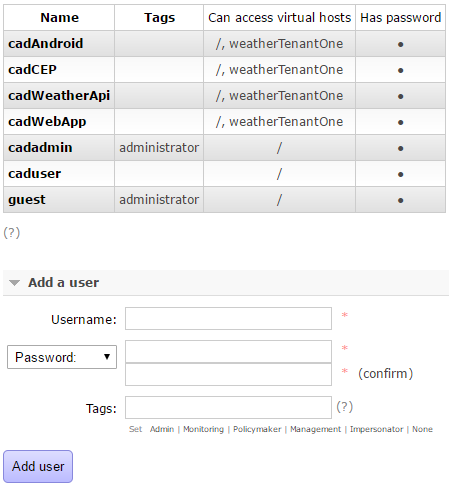
\includegraphics[width=0.5\textwidth]{Bilder/createUser.png}
	\caption{Administrationsmenü zur Benutzererstellung }
	\label{img:AdminCreateUser}
\end{figure}
Die Erstellung neuer Nutzer und die Verwaltung der Rechte erfolgt über unter anderem über das Management Plugin. In Abb. \ref{img:AdminCreateUser} ist ersichtlich, dass die User \textit{cadAndroid}, \textit{cadCEP}, \textit{cadWeatherApi} und \textit{cadWebApp} Zugriff auf den gemeinsamen vHost weatherTenantOne haben. Durch dieses Verfahren kann das gleiche Topic von mehreren Nutzern mit unterschiedlichen vHosts verwendet werden, ohne das sie die Nachrichten anderer vHosts des gleichen Topics lesen können. 
\begin{figure}[htbp]
	\centering
	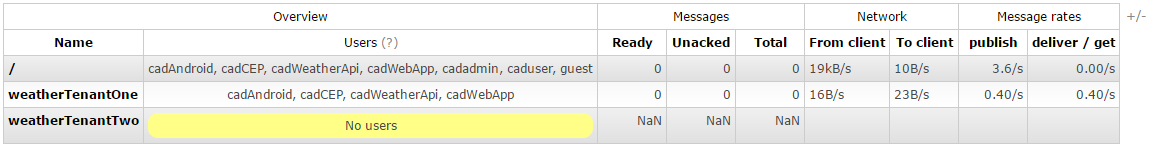
\includegraphics[width=1.0\textwidth]{Bilder/vHostsOverview.png}
	\caption{Übersicht über die virtuellen Hosts}
	\label{img:vHostOverview}
\end{figure}
Eine Übersicht über die einzelnen vHosts und die berechtigten Nutzer wird in Abb. \ref{img:vHostOverview} dargestellt. Diese zeigt noch einmal die erwähnte Zugriffsbeschränkung auf die vier Nutzer dieses Use-Cases sowie den aktuell verursachten Datentransfer der vHosts. Auf diese Weise erfüllt die Anwendung die Anforderung der Multi-Tenancy. Zusätzlich zum Management Plugin bietet RabbitMQ eine HTTP-Schnittstelle. Diese ermöglichen es dem Administrator zum einen über eine Kommandozeile in Verbindung mit Kommandozeilenprogrammen wie cURL (Client for URLs) die angebotenen Schnittstellen aufzurufen und dadurch unter anderem Nutzer anzulegen oder die Verbindungsraten der vHosts auszugeben und auszuwerten (vgl. https://pulse.mozilla.org/api/). Aufgrund der vorhandenen Schnittstellen bietet sich dem Entwickler die Möglichkeit, die Administration über eine eigene Applikation durchzuführen. 

\section{Datenquelle (Wetter-API)}
 



\begin{table}[!ht]
  \centering
    \begin{minipage}{15cm}
      \centering
      \begin{tabular}{*{3}{|l|p{5.0cm}|p{5.0cm}}}\hline
      \multicolumn{4}{|c|}{\cellcolor[RGB]{200,200,200}Validierung nach "12 Faktor APP"} \\\hline
     \textbf{ID}&\textbf{Anforderung}&\textbf{Validierungs Element}&\textbf{Erfüllt}\\\hline
     1.&Codebase&....&Nein\\
      \hline
     2.&Abhängigkeiten&....&Nein\\
     \hline
     3.&Konfiguration&....&Nein\\
     \hline
     4.&Unterstützende Dienste&....&Nein\\
     \hline 
     5.&Build, release, run&....&Nein\\
     \hline
     6.&Prozesse&....&Nein\\
     \hline
      7.&Bindung an Ports&....&Nein\\
     \hline
      8.&Nebenläufigkeit&....&Nein\\
     \hline
      9.&Einweggebrauch&....&Nein\\
     \hline
     10.&Dev-Prod-Vergleichbarkeit&....&Nein\\
     \hline     
     11.&Logs&....&Nein\\
     \hline
     12.&Admin-Prozesse&....&Nein\\
     \hline
      \end{tabular}
   \caption{Validierung nach "12 Faktor APP"}\label{tab:Anforderungen}
    \end{minipage}
\end{table}

ToDo: Verweis auf 12 Faktor APP Standard !!! 




\section{Datenverarbeitung}
\subsection{CEP}
\subsection{Datenbank}



\section{Anwendersicht}
\subsection{Andriod-APP}
\subsection{Web-Client}
\section{Deployment}
\subsection{Allgemein}
\subsection{Cloudfoundry}
\subsection{Docker}
Die in Absatz \ref{rabbitmq} erläuterte message-oriented Middleware RabbitMQ wird als Docker Container deployed. Durch die Verwendung von Docker Containern ist es möglich, lauffähige Software in isolierten Containern zu starten. Dies hat den Vorteil, dass die Software immer in identischen Umgebungen gestartet wird, unabhängig davon ob der Container lokal auf dem Entwicklungsrechner oder auf dem Produktivsystem läuft. Dies betrifft auch die Abhängigkeiten von notwendigen Installationen. So basiert RabbitMQ wie in Absatz \ref{rabbitmq} erwähnt auf der Sprache Erlang, weshalb diese auf jedem Entwicklungs- und Produktivsystem installiert werden müsste. Durch die Verwendung von Docker können notwendige Installationen bereits im Dockerfile definiert werden. So wird beispielsweise die Installation von Erlang in Abb. \ref{img:erlangDockerfile} veranschaulicht. 

\begin{figure}[htbp]
	\centering
	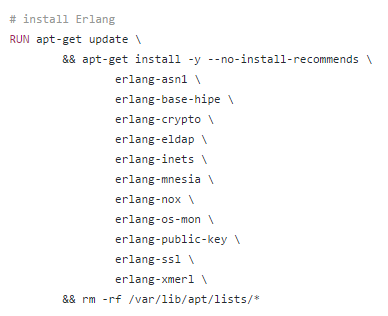
\includegraphics[width=0.5\textwidth]{Bilder/erlangDockerfile.png}
	\caption{Installation von Erlang im Dockerfile Quelle: https://github.com/docker-library/rabbitmq/blob/a6cb36022a5c1a17df78cfafe45a73d941ad4eb8/3.6/\-debian/Dockerfile}
	\label{img:erlangDockerfile}
\end{figure}
Dies ist ein Ausschnitt aus dem Dockerfile des offiziellen Rabbitmq-Baseimages, einer Abbildung des Containers. Der Abschnitt stellt die Installation von Erlang auf einem Linux-System unter Verwendung des Paketmanagers \textit{Advanced Packaging Tool} (APT) dar.
\subsubsection{Dockerfile}
Das Dockerfile für diesen Use-Case besteht neben dem erwähnten Baseimage aus Aktivierungen des in Absatz \ref{rabbitmq} vorgestellten Management Plugins, des MQTT Plugins sowie des MQTT-Websocket Plugins. Durch die Verwendung des Websocket Plugins ist die Kommunikation mit RabbitMQ auch über Webseiten möglich. Ein weiterer Bestandteil des Dockerfiles ist die rabbitmq.config. Diese ist notwendig um den Zugriff auf die MOM einzuschränken, da andernfalls eine Default-Konfiguration verwendet werden würde und durch diese der Nutzer \emph{guest} vollen Zugriff hätte. Um dennoch Administrations-Zugriff zu erlangen, wird über das Shell-Skript \textit{init.sh} ein Nutzer mit Administratorrechten angelegt. Die Zugangsdaten dieses Nutzers sind als Umgebungsvariablen hinterlegt. Die Ausführung des Skripts wird über den CMD-Befehl des Dockerfiles gesteuert. Zusätzlich ist es notwendig, Docker über den Befehl EXPOSE zu informieren, welche Ports der Container abhört. Im Anschluss an die Erstellung des Dockerfiles kann durch den Befehl \emph{docker build} ein Image erzeugt werden. Dieses Image wird auf den Amazon Container Service deployed.
\subsubsection{Amazon Container Service}
Dabei handelt es sich um einen hoch skalierbaren Container Managementservice welcher eine unkomplizierte Handhabung von Docker Containern in Amazon EC2 Instanzen anbietet. Die Erstellung eines Clusters ist in wenigen Schritten möglich. Zunächst wird ein Repository zur Speicherung des erstellten Images angelegt. Im Anschluss daran kann nach der erforderlichen Installation des Amazon Web Service Command Line Interfaces (AWS CLI) der Zugriff auf das Repository erfolgen. Nachdem das Image gepusht wurde, muss die Task Definition erstellt werden. Dabei handelt es sich um eine Anleitung für den Start des Containers. Ein Bestandteil der Task Definition ist das Port Mapping. Dabei wird dem Service mitgeteilt, wie die im Dockerfile deklarierten Ports ausserhalb des Containers erreichbar sein sollen. Zusätzlich werden in den erweiterten Optionen die Umgebungsvariablen und somit die Zugangsdaten für den in der \emph{init.sh} erstellten Administator hinterlegt. Im nächsten Schritt erfolgt die Konfiguration des Services, in welcher ein Load Balancer erstellt und ausgewählt werden kann. Im abschließenden Schritt erfolgt die Konfiguration des eigentlichen Clusters. Hierbei erfolgt die Auswahl der Art und der Anzahl des gewünschten Instanz Typs. Durch diesen wird festgelegt, welche Resourcen für eine einzelne Instanz verfügbar sein werden. Darüber hinaus kann in diesem Abschnitt ein Schlüsselpaar für den SSH-Zugriff erstellt und ausgewählt werden. Erfolgt dies nicht, ist kein Zugriff über die EC2 Konsole auf den Container möglich.



\subsection{REDIS}
\subsection{AWS}


\section{Kostenmodell}


\end{document}
